\subsection{Processing}

The main backbone of this use case is provided by Flink. After the data is being acquired from NiFi into Kafka, it's processed by a Flink application which then will persist enriched data on HDFS, MongoDB and Cassandra.
\\
Before talking about the Flink application per se, it's worth saying that Flink has been deployed on top of YARN with a Job Manager with 1GB of memory allocated and a single Task Manager with 3GB of memory and 3 slots for parallelism, for a total of 4GB and 4 vCPUs allocated on YARN. 

The Flink application has been written in Scala, making use of the appropriate Scala API provided by Flink. The job has been configured to checkpoint every minute, through an externalised checkpoint, to use as a state backend HDFS and use \texttt{EventTime} as the Stream Time Characteristic.

\subsubsection{Application}

\begin{figure}[h]
    \centering
    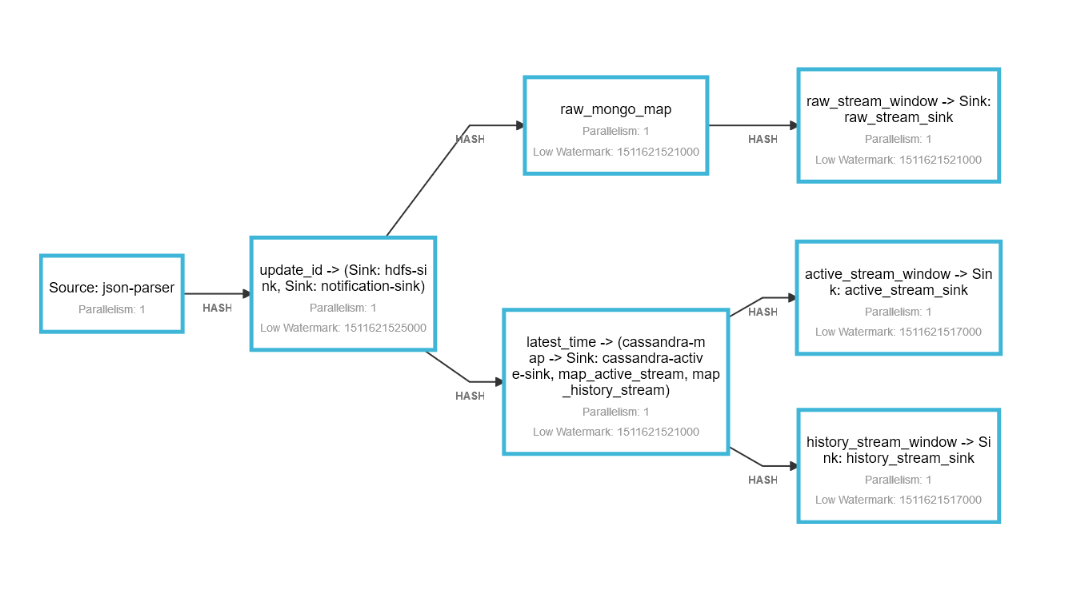
\includegraphics[width=0.8\linewidth]{Figures/flink_job}
    \caption{An overview of the complete DAG of the Flink application described in this section}
    \label{fig:flinkjob}
\end{figure}


\paragraph{Source}
The Flink application has a single source, a Kafka Consumer configured to consume from the \texttt{air\_traffic} topic connecting to both the active kafka brokers on \texttt{master-1} and \texttt{master-2}. Flink's built-in Kafka Consumer must be configured with a deserialization schema, which, in this case, parses from each JSON an \texttt{AirTrafficEvent} using Scala library \href{https://www.playframework.com/documentation/2.6.x/ScalaJson#The-Play-JSON-library}{Play-JSON}.

\begin{code}
   \begin{minted}[breaklines]{Scala}
class JSONDeserializationSchema extends AbstractDeserializationSchema[AirTrafficEvent] {
       
    @throws[IOException]
    override def deserialize(message: Array[Byte]): AirTrafficEvent = {
       
    val obj = Json.parse(message)
    obj.as[AirTrafficEvent]
    }
       
    override def isEndOfStream(nextElement: AirTrafficEvent) = false
}
   \end{minted}
\end{code}

\texttt{AirTrafficEvent} is defined as a Scala case class with three fields wrapping all of the information contained in the original JSON: \texttt{FlightInfo}, containing flight, callsign, registration, origin, destination and aircraft, \texttt{InstantValues}, containing time, altitude, speed and course, and \texttt{Coordinates}, containing latitude and longitude.

\begin{code}
    \begin{minted}[breaklines]{Scala}
//AirTrafficEvent definition
case class AirTrafficEvent
    (flightInfo: FlightInfo,
     coordinates: Coordinates,
     instantValues: InstantValues) extends Event(flightInfo, coordinates, instantValues) with Comparable[AirTrafficEvent]

//FlightInfo definition
case class FlightInfo
    (origin: String,
     destination: String,
     flight: String,
     aircraft: String,
     registration: String,
     callsign: String) extends Serializable

//InstantValues definition
case class InstantValues(speed: Int, altitude: Int, course: Int, time: Date) extends Serializable with Comparable[InstantValues]

//Coordinates definition
case class Coordinates(lat : Double, lon: Double) extends Serializable
    \end{minted}
\end{code}

Since Flink is using EventTime as Time Characteristic of the stream, a timestamp and a watermark should be assigned to every record, in order to be correctly managed for in order consuming and windows. The assigned timestamp and watermark are directly extracted using the \texttt{instantValues.time} field from the parsed \texttt{AirTrafficEvent}, via a \justify{\texttt{BoundedOutOfOrdernessTimestampExtractor}} to make sure that late events within 10 seconds are still correctly processed by Flink.

\paragraph{Operations}

Two main operations are performed on the data flowing through the DAG representing the application: the UID generation of the flight record currently processed and the event processing to get aircrafts which supposedly have arrived to destination.

UID generation is made through \texttt{UpdateIdFunction}, a stateful \texttt{ProcessFunction} processing each element of the stream according to the following pseudo-code:

\begin{minted}{Python}
if is_active_flight(element):
    id = old_id # mantained as state
else:
    id = id + 1
    notify_on_new_flight()
event = event_with_id(element, id)

return event
\end{minted}

It takes as input a \texttt{KeyedStream} of \texttt{AirTrafficEvent}s and outputs an \texttt{AirTrafficEventWithId} stream: the ID is an integer counter which gets increased each time a new instance of a flight is being detected and used to create the actual id of the outputted objects concatenating the flight id with this integer ID (e.g. the first instance of flight \texttt{AZ775} will have id \texttt{AZ775-1}). 

\begin{code}
    \begin{minted}{Scala}
    val streamWithId : DataStream[AirTrafficEventWithId]= stream
        .keyBy(_.flightInfo.flight)
        .process(new UpdateIdFunction())
    \end{minted}
\captionof{listing}{A KeyedStream of AirTrafficEvent processed into an AirTrafficEventWithId stream}
\end{code}

The function handling the detection of a new instance of a flight is based off an heuristic strategy using the latest available information about the position, speed and time of the flight. This is needed because the stream may be inaccurate when it comes to transoceanic flights, passing over dead zones, without any radar at range being able to catch their transponder signals. The heuristic is described by the following Scala snippet:

\begin{minted}[breaklines]{Scala}
val activeUpperBound = Time.minutes(5) // 5 minutes
val notActiveLowerBound = Time.hours(5) // 5 hours
val threshold = Time.minutes(120) // 60 minutes
val (last_lat,last_lon) = lastKnownPosition.value match {
    case null => return false
    case _ => lastKnownPosition.value
}
val last_speed = lastSpeed.value  match {
    case 0 => return false
    case _ => lastSpeed.value
}
val last_time = lastTime.value  match {
    case 0 => return false
    case _ => lastTime.value
}

if(new_time - last_time < activeUpperBound.toMilliseconds) true
else if(new_time - last_time > notActiveLowerBound.toMilliseconds) false
else
    Math.abs(distFrom(new_position, (last_lat, last_lon))/knotsToMetersSeconds(last_speed)
        - (new_time - last_time)/1000) < threshold.toMilliseconds/1000

\end{minted}

in which can be seen that there are three main conditions being checked:
\begin{enumerate}
    \item if the difference between the timestamps is less than a certain upper bound (default 5 minutes), meaning that we received an event from the current flight recently and implying the it is active.
    \item if the difference between the timestamps is greater than a certain lower bound (default 5 hours), meaning that we haven't received an event from the current flight in a while, implying it's a new instance of a flight. This case is used as a discriminant for flights flying over dead zones.
    \item provides a prediction based off the estimated time to reach the latest position from the previous last known position, at constant speed=last\_speed, and the actual time taken to reach the latest position.
\end{enumerate}

This way, we are able to be reasonably certain that an aircraft, even after passing over a dead zone for more than 5 minutes, is still flying towards its destination and we are not dealing with another instance of the same flight. A more accurate heuristic would be possible with a data source not cutting under 37000 feet and using an additional data source with the airports and their position, integrated within the stream structure.

Additionally, whenever a new instance of a flight is detected a side-output is used to forward outside of the \texttt{ProcessFunction} an \texttt{Alert} containing the relevant event, together with the event type, which is, in this case, \texttt{newAirplane}.
\\\\
Just like it has been mentioned, the second operation executed on the stream concerns the event processing used to detect aircrafts arriving to their destination. Since it's been noted that the data stream is incomplete, in order to demonstrate \textbf{FlinkCEP} capabilities when it comes to event processing, instead of using a pattern that detects variations in altitude and speed to correctly determine the sequence of events implied by an aircraft approaching to an airport, it's been used a simple pattern based on the timing out of events sequences.

The pattern is implemented as follows:

\begin{minted}{Scala}
val airplaneArrivalPattern = 
Pattern
    .begin[AirTrafficEventWithId]("flying")
        .where(_.airTrafficEvent.instantValues.altitude >= 37000)
        .oneOrMore
    .notNext("disappearing")
        .where(_.airTrafficEvent.instantValues.altitude >= 37000)
        .within(Time.minutes(30))

// Associate KeyedStream with pattern to be detected
val patternStream  = CEP.pattern(streamById, airplaneArrivalPattern)
//Side output where timed out events are forwarded
val outputTag : OutputTag[Alert] = OutputTag[Alert]("side-output")
// How to handle timed out and in-time events
val result: DataStream[AirTrafficEventWithId] = 
    patternStream.select(outputTag) { //Timed out events
        (pattern: Map[String, Iterable[AirTrafficEventWithId]], 
        timestamp: Long) => {
            val alert = new Alert(pattern("flying").last, 
                                  AlertType.disappearedAirplane.id)
            alert
        }
    } { //In time events
        (pattern: Map[String, Iterable[AirTrafficEventWithId]]) =>
            pattern("flying").last
    }   
// Collect timed out events from the main stream
val alertStream = result.getSideOutput(outputTag)
alertStream
    .addSink(new NotificationSink())
    .uid("notification-sink")
    .name("notification-sink")
\end{minted}

and is basically structured on the analysis of a Keyed Stream, keying on the event id, such that if there's no event within 30 minutes from the last one, the pattern times out, an \texttt{Alert} is created, from the last event stored, and then forwarded to the notifications' sink.

\paragraph{Sinks}

The Flink application has three main sinks where data is forwarded to be stored after processing: \textbf{MongoDB}, \textbf{Hive via HDFS} and \textbf{Cassandra}. On these three sinks there are three types of data stores: a \textit{raw} data store where all the records are saved after being enriched with their unique ID, an \textit{history} data store where it is saved a single record per flight, updated as needed, and an \textit{active} data store used for live monitoring purposes. An additional sink is used for the \texttt{Alert}s constructed during the stream processing.

\textbf{MongoDB} is used as sink for all of the three data stores, with adequately defined collections, while \textbf{Cassandra} is used for the \textit{active} data store, and \textbf{Hive} via HDFS is used only for the \textit{raw} and \textit{history} ones.
\\\\
Cassandra Sink in Flink is added through the \texttt{CassandraSinkBuilder} used to specify the query to be used while inserting the records in the table:

\begin{minted}{Scala}
// Add sink to Cassandra cluster
CassandraSink.addSink(
    airtrafficEvents
        .map(_.toCassandraTuple)
        .javaStream)
.setQuery(
    s"""UPDATE air_traffic.active
    |SET lat = ?, lon = ?, speed = ?,
    |    altitude = ?, course = ?, flight = ?,
    |    origin = ?, destination = ?, aircraft = ?, time = ?
    |    WHERE id = ?;""".stripMargin)
.setClusterBuilder( new ClusterBuilder {
def buildCluster(builder: Cluster.Builder): Cluster = {   
    builder.addContactPoint("slave-1")
    builder.addContactPoint("slave-2")
    builder.addContactPoint("slave-3")
    builder.addContactPoint("slave-4")
    builder.build()
}
}).build()
\end{minted}

On Cassandra's cluster, composed as already mentioned previously, by the four slave nodes, has been specified an \texttt{air\_traffic} keyspace, configured with a replication factor of 3 via the replication strategy \texttt{SimpleStrategy}. Within this keyspace the following table has been defined:

\begin{minted}{SQL}
CREATE TABLE air_traffic.active (
    id text PRIMARY KEY,
    altitude int,
    course int,
    destination text,
    flight text,
    aircraft text,
    lat double,
    lon double,
    origin text,
    speed int,
    time timestamp
) WITH default_time_to_live = 600
       AND gc_grace_seconds = 3600
\end{minted}

in order to contain all of the active aircrafts currently flying. All of the default configurations have been maintained, except for the TTL of the records which has been configured to 10 minutes and the interval of the garbage collection of the table tombstones (expired records after the TTL) which has been set to 1 hour, instead of 1 day.
\\\\
Notifications sinks are rather simple \texttt{SinkFunction}s which take as input the \texttt{Alert} and make an async \texttt{POST} request, through a \href{https://dispatchhttp.org/Dispatch.html}{Dispatch} asynchronous HTTP client, to the local notification server, implemented using Firebase FCM, about which we'll talk about later on.
\\\\
Hive is not the direct destination of the Flink sink. As a matter of fact, an HDFS sink is used to write all of the records in JSON format, partitioned in folders according to their timestamp. As a result, each event will be bucketed in the appropriate folder and this folder will be considered as a partition of an Hive external table configured using the \textbf{JsonSerDe} to read all of the files.

\begin{minted}{Scala}
val hdfsSink = new BucketingSink[AirTrafficEventWithId](hdfs_path)
hdfsSink.setBucketer(new EventDateTimeBucketer("YYYY-MM-dd"))
hdfsSink.setBatchSize(1024 * 1024 * 64) // 64MB files size

streamWithId.addSink(hdfsSink).uid("hdfs-sink").name("hdfs-sink")
\end{minted}

while the Hive external table is defined as it follows:

\begin{minted}[breaklines]{SQL}
CREATE EXTERNAL TABLE IF NOT EXISTS json_dump
( `origin` string,
`flight` string,
`course` int,
`aircraft` string,
`callsign` string,
`registration` string,
`lat` double,
`lon` double,
`altitude` int,
`speed` int,
`destination` string,
`time` timestamp,
`_id` string)
PARTITIONED BY (`dt` string)
ROW FORMAT SERDE 'org.apache.hive.hcatalog.data.JsonSerDe'
WITH SERDEPROPERTIES ('timestamp.formats'='YYYY-MM-dd HH:mm:ss.SSS')
STORED AS TEXTFILE
LOCATION '/flink/air_traffic/json_dump';
\end{minted}

Starting from this very table, which maintains records in text format, uncompressed, further optimizations will be performed before the final storage within Hive.

\subsubsection{Post-processing: HDFS to Hive}

As we already determined, Hive is not the direct target of Flink, since we're using an Hive external table to read all of the Json files written by the HDFS sink. Using a textfile format is not optimal for storage purposes, since it's not a compressed format and we'd like to save as much storage as possible. For this reason an additional table, in the appropriate database in Hive, has been defined to be the final target of the raw stream written in HDFS. Additionally, from this table, another table called history is filled, aggregating all of the records of a flight in a single record with arrival date and departure date.

To sum up, there are three tables stored in Hive:
\begin{itemize}
    \item \texttt{json\_dump}, external table reading the Json files written by Flink;
    \item \texttt{raw} in \texttt{air\_traffic} database, containing an optimized version, for storage and query purposes, of \texttt{json\_dump} 
    \item \texttt{history} in \texttt{air\_traffic} database, aggregating \texttt{raw} creating a single record for each flight.
\end{itemize}

The raw table is defined to use ORC as storage format, to use Hive partitioning on the date and to be clustered in 100 buckets, in order to make sure that, if needed, a query concerning a certain subset of flights wouldn't read all of the files composing the table.

\begin{minted}[breaklines]{SQL}
CREATE TABLE IF NOT EXISTS air_traffic.raw(
`origin` string,
`flight` string,
`course` int,
`aircraft` string,
`callsign` string,
`registration` string,
`lat` double,
`lon` double,
`altitude` int,
`speed` int,
`destination` string,
`time` timestamp,
`_id` string)
PARTITIONED BY (`dt` string)
CLUSTERED BY (flight) INTO 100 BUCKETS
STORED AS ORC;
ALTER TABLE air_traffic.history SET SERDEPROPERTIES("timestamp.formats"="YYYY-MM-dd HH:mm:ss.SSS");
\end{minted}

The history table is instead defined with the additional fields \texttt{arrival\_date} and \texttt{departure\_date}, removing all of the instant values, deemed as not needed, as it follows:

\begin{minted}{SQL}
CREATE TABLE `history`(
`_id` string, 
`date_depart` timestamp, 
`date_arrival` timestamp, 
`flight` string, 
`callsign` string, 
`registration` string, 
`aircraft` string, 
`origin` string, 
`destination` string)
PARTITIONED BY (`dt` string)
\end{minted}

Both these tables are filled in a periodic batch operation, scheduled every 20 minutes, through \texttt{INSERT OVERWRITE} queries on the current partition (date): whereas the \texttt{raw} is a simple overwrite from \texttt{json\_dump} as they have the same schema,  \texttt{history} aggregates the time field via \texttt{MAX()} and \texttt{MIN()} Hive aggregated functions as shown below:

\begin{minted}{SQL}
INSERT OVERWRITE TABLE air_traffic.history 
PARTITION(dt="${PARTITION}")
(SELECT
    `_id`,
    MIN(time) AS date_depart,
    MAX(time) AS date_arrival,
    flight,
    callsign,
    registration,
    aircraft,
    origin,
    destination
FROM air_traffic.raw
WHERE dt="${PARTITION}"
GROUP BY 
    `_id`,
    flight,
    callsign,
    registration,
    aircraft,
    origin,
    destination)
\end{minted}

Periodic scheduling has been set using \texttt{crontab} functionalities of CentOS, which is used to execute a Python script called \texttt{hive\_loader} which executes the needed queries. \texttt{Hive\_loader} has four flags used to determine which queries has to be executed:
\begin{enumerate}
    \item \texttt{bootstrap}, which creates all of the tables used.
    \item \texttt{update}, which controls the scheduled execution for the update of raw and history tables.
    \item \texttt{add\_partition\_update}, used after midnight to definitively update \texttt{raw} and \texttt{history} of the previous day, while adding a new partition to \texttt{json\_dump}.
    \item \texttt{drop\_partition}, used to drop the previous day partition, before deleting it.
\end{enumerate}

Together with the aforementioned tables, additional tables have been created and filled to be available to Tableau for visualisation purposes:

\begin{itemize}
    \item \texttt{aircrafts}, containing the ID model and its capacity in terms of number of passengers.
    \item \texttt{airports}, containing, for each airport, its complete name, its IATA code, its continent and its ISO country and region codes.
\end{itemize}